\epigraph{\textit{We cannot solve problems with the kind of thinking we employed when we came up with them.}}{-- \textup{Albert Einstein}}

During the following paragraphs I am covering the motivation, contributions and structure of this document. This means, after reading it, you are building the big picture; a general idea of the motivations to develop this project, the results we are looking for and the shape of it.

\section{Motivation}

A famous mathematical problem from the past is \textbf{The Seven Bridges of Königsberg}. The foundations of \textit{graph theory} were set by Leonhard Euler's negative solution to the problem in 1736.

The city of Königsberg in Prussia (now Kaliningrad, Russia) was built on both banks of the Pregel river and featured two sizable islands, Kneiphof and Lomse, which were linked to the two mainland sections of the city by seven bridges. Creating a route through the city that would cross each of those bridges just once was the challenge. What Euler proved was that this problem has no solution.

\begin{figure}[ht]
    \begin{subfigure}{.3\textwidth}
        \centering
        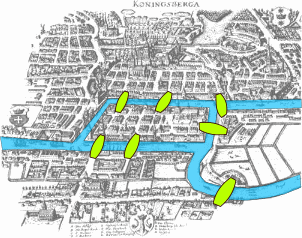
\includegraphics[width=.7\linewidth]{img/1-1_konigsberg_bridges.png}
        \caption{The seven bridges' exact positioning is shown on Königsberg's map from Euler's time, highlighting the Pregel river in blue}
    \end{subfigure}%
    {\LARGE$\rightarrow$}%
    \begin{subfigure}{.3\textwidth}
        \centering
        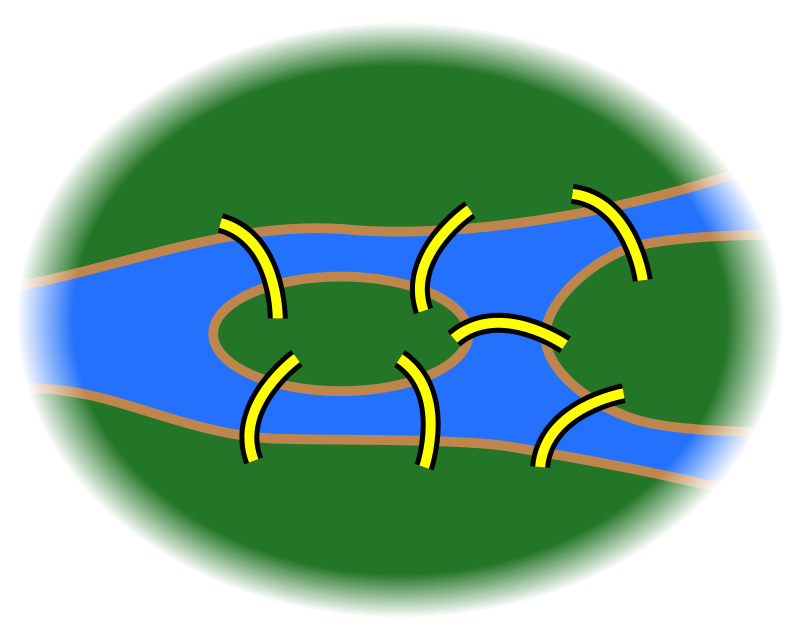
\includegraphics[width=.7\linewidth]{img/1-2_konigsberg_abstract.png}
        \caption{Diagram illustrating The Seven Bridges of Königsberg's puzzle. Take note of how our level of abstraction has increased}
    \end{subfigure}%
    {\LARGE$\rightarrow$}%
    \begin{subfigure}{.3\textwidth}
        \centering
        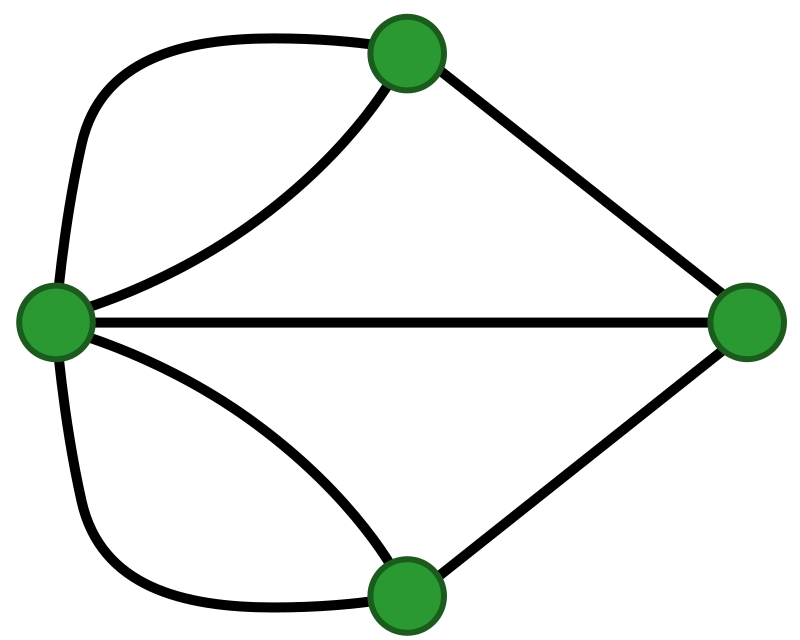
\includegraphics[width=.7\linewidth]{img/1-3_konigsberg_graph.png}
        \caption{Abstract graph corresponding to the bridges of Königsberg, where edges are de bridges and nodes are the sector of the city}
    \end{subfigure}%
    \caption[Creating the equivalent graph of the problem of The Seven Bridges of Königsberg]{Creating the equivalent graph of the problem of The Seven Bridges of Königsberg\footnotemark}
\end{figure}
\footnotetext{\url{https://en.wikipedia.org/wiki/Seven_Bridges_of_Konigsberg}}

\subsection{Eueler's analysis}

In modern terms, Euler made the observation that the degree, number of vertices connected to a particular element, of the nodes, determines the possibility of a walk around a graph, traversing each edge precisely once. According to Euler's theory, a connected graph with exactly zero or two nodes with odd degrees is a requirement for the walk around the entire network. This is due to the fact that we can only cross each bridge once, therefore each traversal of a section of the city requires an even number of edges to be crossed. For each entrance on a mainland, we must enter through one bridge and exit through another. It turns out that this condition is also sufficient. We also know that if there are nodes with odd degrees, then any path will begin at one of them and end at the other. A path like this is currently known as the Eulerian path and is named after the mathematician. There can be no Eulerian path in the graph that corresponds to Königsberg since it contains four nodes of odd degree.

\section{Project Scope}

A growing number of devices are interconnected, these days. As a result, a ton of data is being automatically stored. This way, processing that data becomes both a more challenging procedure and a more important task. Simply stated, the amount of data outruns our capacity to consume it. Big data, a new area of software development where we quickly handle large volumes of heterogeneous information, offers a remedy for this.

Interoperability is a crucial subject we must deal with in big data applications since they not only need to scan huge volumes of inputs as quickly as possible but also because information comes from a range of sources.

Knowledge graphs~\cite{https://doi.org/10.48550/arxiv.2110.11709} were popularized back in 2012 by Google~\cite{web:knowledge_graphs:google} as a tool to represent real world data reflecting relationships between entities in order to understand those links better. After Google's introduction, others embraced this approach: ranging from proprietary to open databases. Being the content of the latter publicly available. Prominent companies -- including \textit{web search} (e.g., Bing~\cite{knowledge:graphs:usage:bing} and Google~\cite{web:knowledge_graphs:google}), \textit{commerce} (e.g., Airbnb~\cite{knowledge:graphs:usage:airbnb} and Amazon~\cite{knowledge:graphs:usage:amazon}), \textit{social networks} (e.g., Facebook~\cite{knowledge:graphs:usage:facebook} and LinkedIn~\cite{knowledge:graphs:usage:linkedin}) or \textit{finances} (e.g., Accenture~\cite{knowledge:graphs:usage:accenture} and Banca d'Italia~\cite{https://doi.org/10.48550/arxiv.2010.05172}) -- are using knowledge graphs in order to have a better understanding of their customers. Even though there exist several models associated with this technology, we are focusing on Wikibase graphs.

Summing up, this project focuses on the analysis and implementation of a system to validate Wikibase graphs -- a specific flavor of the so-called knowledge graphs -- using big data techniques. To put that into perspective, as of October 1, 2022, a compressed \gls{dump} of Wikidata's database has a size of 109.04Gb~\cite{wikidata:dumps}. Not only that, but the size of these dumps has exponentially increased with each and every release of a new one (see Figure \ref{fig:dumps}).

\begin{figure}[ht]
    \centering
    \includestandalone[width=0.4\textwidth]{diagrams/1-1_dumps}
    \caption[Plot showing the size of compressed dumps between 2014-22]{Size of compressed Wikidata dumps between 2014-2022~\cite{https://doi.org/10.48550/arxiv.2110.11709}}
    \label{fig:dumps}
\end{figure}

These enormous sizes have the effect of making it difficult for users to easily examine and process the content, and they also raise the possibility that these technologies will become victims of their own success. This condition is demonstrated in Scholia, an online application that uses Wikidata to describe data about academics and their works. Additionally, the app includes appealing visualizations and comparisons that are based on requests through the Wikidata endpoint. Despite the project offering a wealth of intriguing data, timeouts caused by the massive volumes of data prevent access to the most intricate visualizations.

Creating subsets of the Knowledge Graphs for specific domains may be one solution to these problems. These subsets serve as snapshots of the data at certain points in time and be used to enhance the performance of the apps that use that data, making it easier to do research on the contents of Knowledge Graphs.

\section{Objectives}

\paragraph{Project's Goal 1}
\textit{Design and implementation of a system for validating huge dumps from Wikidata generating a subset out of it.} As we have stated during these introductory lines, the task of having to process enormous amounts of data is becoming increasingly relevant. The faster a system allows us to accomplish it, the better solution we will provide.

\paragraph{Project's Goal 2}
\textit{Reproduce an experiment related to the analysis of the previously described algorithm.} In order us to properly analyze the results emerging from the execution of the algorithm we have implemented, we have to create an ecosystem were we can obtain information related to memory consumption or execution time, to name a few.

\paragraph{Project's Goal 3}
\textit{Learn new technologies and Big data techniques.} This is an academic project, not only that, but one of the main objectives of researching is finding new solutions to a certain problem. This means, learning and exploring new possibilities is -- indeed -- one goal of this project.

\section{Contributions}

The main contributions of this project are:

\begin{enumerate}
    \item
\end{enumerate}

\section{Structure of the document}

The shape of this document is as follows:

\begin{itemize}
    \item \textbf{Chapter ~\ref{chapter:related}.} General description of the existing technologies related to knowledge graph validation. As well as the advantages and disadvantages of choosing some tools over others for implementing this project.
    \item \textbf{Chapter ~\ref{chapter:theory}.} Provides a theoretical background needed for better understanding the concepts explained in the following chapters.
    \item \textbf{Chapter ~\ref{chapter:experiment}.} Explanation of the process followed to analyze the concrete implementation of the algorithm that we used to validate the knowledge graphs.
    \item \textbf{Chapter ~\ref{chapter:results}.} Analysis of the results obtained from the previously described experiment.
    \item \textbf{Chapter ~\ref{chapter:conclusions}.} Summary of the general conclusions and future work.
\end{itemize}